\section{OpenCV}

\begin{figure}[htbp]
\centering

\includegraphics[width=0.3\textwidth]{images/openCV/opencv-logo.png}
\end{figure}


\textbf{OpenCV} (“Open Source Computer Vision Library”) è una libreria open source che offre funzionalità per applicazioni di computer vision.

\subsection{Storia}
Il progetto OpenCV è stato lanciato nel 1999 dalla Intel come una parte di varie iniziative volte a sviluppare applicazioni ad elevata efficienza.\cite{opencv1}

La versione alpha è stata rilasciata nel 2000 mentre successivamente sono state rilasciate varie versioni beta; il rilascio della versione 1.0 è avvenuto
nel 2006.

Dal 2008 il progetto è supportato dalla casa di produzione e ricerca \textbf{Willow Garage}, che si occupa di sviluppo di hardware e software open source per applicazioni robotiche. Nel 2009 è stata rilasciata una versione più efficiente, caratterizzata da migliori implementazioni e più funzionalità, delle quali una è la possibilità di parallelizzare il lavoro nei sistemi multi-core.

\subsection{Computer vision}

La \textbf{computer vision} è una disciplina che ha come obiettivo principale ricreare la vista umana, utilizzando metodi per analizzare e processare immagini dal mondo reale al fine di estrapolarne determinate informazioni \cite{vision,vision2}. Un sistema di computer vision opera in diverse fasi:
\begin{itemize}
\item acquisizione immagini tramite supporti ottici come telecamere.
\item digitalizzazione dell'immagine.
\item elaborazione dell'immagine da parte di software, tramite algoritmi per rendere più marcate determinate caratteristiche, in modo da rendere più efficiente il riconoscimento (ad esempio aumentando il contrasto per rilevare meglio i contorni di oggetti).
\item decisione da parte del sistema di scegliere o scartare il campione analizzato, in base allo scopo dell'applicazione, e raccolta di determinate informazioni derivate dall'analisi.
\end{itemize}
I sistemi di computer vision sono sfruttati in moltissimi campi:

\begin{itemize}
\item controllo dei processi industriali: riconoscimento di prodotti, lettura di codici ed etichette, controllo dei nastri trasportatori e della merce, posizionamento ed orientamento di bracci meccanici.
\item riconoscimento di eventi (esempio nella videosorveglianza).

\item controllo di macchine autonome (robot, veicoli di vario genere ed, esteso al campo militare, droni, missili autoguidati etc).

\item medicina: nelle analisi di immagini derivate da ecografie, radiografie e simili, per diagnosticare determinate malattie o rilevare la presenza di tumori.

\item neurobiologia: lo studio della struttura del cervello con la computer vision permette di classificare determinati comportamenti o altre caratteristiche dell'uomo o degli animali.
In particolare nell'ultimo secolo sono stati condotti studi sugli occhi, sui neuroni e sulla struttura del cervello, per studiare i processi del sistema visivo. 

\end{itemize}

\subsection{Video Tracking}
Il \textbf{Video Tracking} consiste nell'individuare un oggetto e tracciare il suo movimento, dato un qualsiasi stream video, come la ripresa di una telecamera. I frame del video vengono processati in modo da rilevare nel tempo la posizione dell'oggetto, o degli oggetti in questione. 

Il problema maggiore di questa tecnica si riscontra nel calcolare con una buona precisione la posizione dell'oggetto in ogni frame.
Questo è dovuto a varie motivazioni:
\begin{itemize}
\item elevata velocità dell'oggetto rispetto al frame rate.
\item qualità della telecamera.
\item fattori ambientali quali luminosità, presenza di ostacoli o falsi positivi che possono interferire con il tracciamento.
\item qualità del \textbf{classificatore} (“cascade”) utilizzato per riconoscere l'oggetto.
\end{itemize}

Tranne le prime due motivazioni, le altre dipendono dal classificatore, un file XML che contiene varie informazioni per riconoscere determinati oggetti in un'immagine. 

\subsection{Il training del classificatore}
In OpenCV esistono delle funzioni per addestrare classificatori, utilizzando vari algoritmi. Il \textbf{training} (“addestramento”) richiede una serie di immagini contenenti l'oggetto da rilevare, chiamate positivi, e una serie di immagini che non contengono l'oggetto in questione, chiamate negativi. In base all'algoritmo utilizzato vengono analizzati i positivi per ricavare le somiglianze, inoltre questi sono confrontati con i negativi per evidenziare le differenze.

Il processo di training richiede tempi lunghi, in quanto, per produrre buoni classificatori, necessita di una grande quantità di immagini di buona qualità. I positivi dovrebbero raffigurare l'oggetto in ogni stato possibile, ovvero visto da ogni angolazione, in ogni sua variante, con presenza di una certa illuminazione, etc. Ad esempio se si vuole addestrare un classificatore per riconoscere volti umani, i positivi dovrebbero raffigurare volti di persone di ogni età, sesso, razza, caratteristiche specifiche quali capelli, barba, occhi, etc, e dovrebbero essere inquadrati da ogni angolazione possibile.

Ovviamente, più è complesso l'oggetto da riconoscere, e più lungo e dispendioso è il processo di addestramento. Questo processo non è banale, basti pensare che all'inizio del progetto si è cercato di creare un classificatore di mandarini (quindi un oggetto molto semplice) e, utilizzando circa 300 positivi e 2000 negativi, con un addestramendo di una ventina di ore, il risultato era di scarsa qualità.

OpenCV offre dei classificatori già addestrati, da utilizzare per le proprie applicazioni.
%Ai fini della nostra applicazione è necessario utilizzare un classificatore per il riconoscimento di volti. Tra i classificatori già addestrati si è scelto di utilizzare il \texttt{haarcascade\_frontalface\_default.xml}, non per motivi di qualità, dato che davano tutti risultati simili, ma perchè si	 è notato da vari esempi trovati in rete che questo è il classificatore più usato.

\subsection{Face Recognition}
I classificatori sono addestrati tramite diversi algoritmi; ognuno ha le sue caratteristiche e può produrre risultati diversi, dato uno stesso insieme di input. Per il riconoscimento del volto (“Face Recognition”) i principali algoritmi sono:

\begin{itemize}
\item \textbf{PCA} (“Principal Component Analysis”): due immagini, supponiamo di risoluzione $100\times100$, formano uno spazio vettoriale di $10.000$ dimensioni, perciò il carico di lavoro per il confronto sarebbe insostenibile.\\
Questo metodo permette di ridurre le dimensioni dello spazio vettoriale prendendo in considerazione solamente le componenti principali, cioè quelle con la massima varianza.
Queste componenti sono chiamate \textit{“eigenfaces”} (da “eigenvalue” = “autovalore”), in quanto il metodo prevede il calcolo di autovettori ed autovalori.\\
Il difetto principale di questo metodo è che risente fortemente di rotazioni o traslazioni, ed è influenzato dall'illuminazione e dall'ambiente.

\item \textbf{LDA} (“Linear Discriminant Analysis”): come nella PCA anche in questo metodo vengono diminuite le dimensioni del sottospazio vettoriale; il miglioramento rispetto al metodo precedente sta nel fatto che le componenti vengono suddivise in classi in cui la varianza è minima. In questo modo classi simili sono vicine tra loro nello spazio vettoriale, mentre classi diverse sono allontanate il più possibile le une dalle altre. Nella PCA può succedere che alcune componenti importanti vengano scartate, in quanto alterate da fattori come la luce o una rotazione del volto. Nella LDA invece, essendo le componenti suddivise in classi, quelle discriminanti vengono mantenute anche in presenza di piccole alterazioni, e questo permette un riconoscimento più efficiente, anche se il volto è ruotato o non è del tutto visibile dalla telecamera.

\item \textbf{Wavelet}: le wavelet sono delle funzioni utilizzate specialmente in analisi armonica, che, tra i vari scopi, permettono di creare dei filtri. Una famiglia di queste trasformate, chiamata \textit{Haar wavelet}, dal suo creatore \textbf{Alfred  Haar} (1909)\cite{haar-wavelet}, ha la caratteristica di avere un dominio di numeri interi compreso tra -1 e 1.\\
\textbf{Paul Viola} e \textbf{Michael Jones} \cite{viola-jones} introdussero l'utilizzo di queste trasformate nel campo del riconoscimento facciale. Il loro sistema utilizza le cosiddette \textbf{Haar-like features} per riconoscere zone con determinate caratteristiche in un'immagine\cite{haar-features}.\\
Un' Haar-like feature è un rettangolo suddiviso in diverse aree, in modo da formare un pattern che deve essere riconosciuto nell'immagine. Ogni feature rappresenta la differenza della somma dei pixel delle varie regioni nel rettangolo. Nel processo di addestramento si parte con delle feature di base, per riconoscere semplici spigoli o contorni. Nella figura \ref{features} si possono osservare alcuni tipi di feature di base \cite{opencvTut2}.\\
\begin{figure}[htbp]
\centering
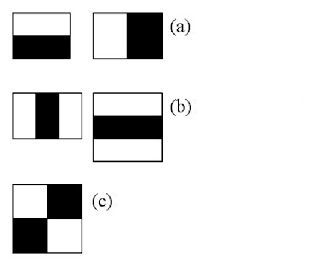
\includegraphics[width=0.5\textwidth]{images/openCV/haar_features2.jpg}
\caption{Alcune haar-features.
			(a): Edge Features.
			(b): Line Features.
			(c): Four-rectangle features.\label{features}}
\end{figure}

Le immagini vengono scansionate alla ricerca dei vari pattern di base. Ad ogni passaggio la ricerca viene ripetuta aumentando le dimensioni dei pattern. Il numero totale di features calcolabili è molto grande, basti pensare che in un'immagine $24\times 24$ è possibile trovare più di $160.000$ features. Per questo si procede a prendere in considerazione solamente le features più rilevanti.
Per esempio nella figura \ref{volti} notiamo che nel volto sono stati riconosciute due particolari features: una all'altezza degli occhi e una che ricalca la forma del naso.
\begin{figure}%[htbp]
\centering
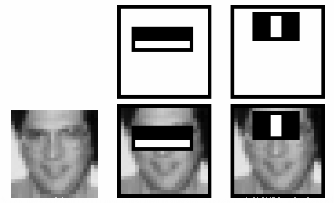
\includegraphics[width=0.5\textwidth]{images/openCV/haar.png}
\caption{Particolari features riconosciute nel volto.\label{volti}}
\end{figure}
Infatti la zona degli occhi solitamente è più scura rispetto alle altre parti del volto, ricalcando il primo pattern di tipo (a) nella figura \ref{features}, mentre il naso, posizionato tra le due zone scure degli occhi, presenta un pattern che ricalca la prima feature di tipo (b).

Dato un insieme di immagini positive, l'algoritmo procede a fare una classificazione per suddividere le features simili in classi uguali, con una soglia prestabilita. Si selezionano solamente le features con rapporto di errore minimo, in modo da suddividere quelle che possono ricondurre alle caratteristiche di un volto da quelle che non fanno parte di esso. Le immagini vengono scansionate fino a che il tasso di errore rimane sotto una certa soglia oppure in base al numero di stages di classificazione deciso dall'utente. Alla fine del processo tutti i risultati, ovvero le features ottenute, vengono salvati all'interno di un file XML, che rappresenta il classificatore desiderato.

OpenCV offre un metodo, \texttt{detect\_multiscale()}, che permette di riconoscere oggetti, scansionando un'immagine con lo scopo di cercare le features descritte nel classificatore. 


\end{itemize}
\clearpage